\clearpage
\section{Forschungsgrundlage}
\label{sec:research}

\subsection{Computational Thinking}

\subsubsection{Definition}
Der Begriff Computational Thinking (CT) wurde erstmals 1980 verwendet \cite{papert}, schlussendlich allerdings erst 2006 wieder weitläufig durch eine Kolumne in den öffentlichen Diskurs gebracht \cite{wing2006}.
Grund der erneuten popularisierung des Begriffes war unter anderem die Diskussion con CT in Kontext von Schulcurricula, und die Wichtigkeit des Konzeptes im Alltag.
Aufgrund dessen, dass es keine allgemein akzeptierte, einheitliche Definition des CT gibt, wurden sich im Kontext der Arbeit verschiedenste Studien betrachtet und verglichen. Es wurde sich für einheitliche Definitionen an einer Review Studie aus dem Jahre 2017 orientiert, die bisherige Forschungsergebnisse abwägt und vergleicht \cite{schute}.
\\
In den frühesten Definitionen von CT wird das Konzept häufig beschrieben als Grundlage für alle unsere Prozesse im Alltag. CT ist demnach nicht nur eine Fähigkeit, die nützlich für Entwickler ist, sondern begegnet uns überall im Alltag \cite{khine17}. Besonders frühere Berichte stellen hervor, dass Computer Science (CS) nicht nur bedeutet, dass man Programmieren kann, sondern dass man Kompetenzen erwirbt, die sich auch in allen anderen Bereichen, sogar künstlerischen Feldern, anwenden lassen \cite{wing2006}.
Auch wird der Begriff im Kontrast zu mathematischem Denken gestellt, und besonders welche Unterschiede und Gemeinsamkeiten die beiden Konzepte haben.

\subsubsection{Computational Thinking Aspekte}
Aufgrund dessen, dass es keine einheitliche Definition von CT gibt, wurden im Rahmen der Arbeit verschiedenste Papers zum Thema analysiert. 2017 wurde eine einheitliche Definition der Aspekte des CT, sowie ein Vergleich aller bisherigen CT Studien von V.J Schute \cite{schute} veröffentlicht, an der sich größtenteils in dieser Arbeit orientiert wird.
Trotz dessen, dass es viele verschiedene Definitionen von CT gibt, kommen diese letztendlich doch auf ähnliche Ergebnisse. Vier Aspekte des CT werden demnach immer wieder erwähnt \cite{schute}.

\begin{description}
    \item[Dekomposition] Todo.
    \item[Abstraktion] Im urspränglichem Paper von M. Wing wird Abstraktion als eine Kernbasis für CT genannt. Hierbei fließt ein weiterer Aspekt ein, die Verallgemeinerung.
    Demnach muss man demnach in der Lage sein, ein komplexes Problem oder System abstrahieren zu können, und auf wesentliche Aspekte zu reduzieren. Wing unterscheidet zudem zwischen Abstraktion in jeweiligen Ebenen, Abstraktion als Ganzes, und Verbindung zwischen den Ebenen. \cite{wing2008}.
    \item[Algorithmen] Je nach Forscher wird dieser Aspekt auch als Algorithmisches Denken bezeichnet, und soll sich so unter Anderem von anderen Denkweisen, wie beispielsweise dem mathematischem Denken abheben \cite{schute}. Weitere Denkweisen, die mit CT verbunden werden können, sind Wissenschaftliches, sowie Logisches Denken \cite{curzon}.
    \item[Debugging] Dieser Aspekt wird auch teilweise als Evaluation \cite{curzon} oder Systematisches Testen \cite{wing2006} bezeichnet. Er beschreibt die tatsächliche Analyse der gefundenen Lösung. Debugging kann zudem dabei helfen, die Lösung zu verallgemeinern, damit diese wieder auf zukünftige Probleme angewandt werden kann.
\end{description}

Es wird zudem argumentiert, dass es noch weitere Aspekte gibt, die für CT allgemein relevant sind \cite{curzon}. Diese Aspekte können teilweise unter dem bereits genannten einsortiert werden.

\begin{description}
    \item[Menschliches Denken] Neben Algorithmischen, Logischem und Wissenschaftlichem Denken, gibt es laut Curzon und McOwan \cite{curzon} noch den abstrakteren, menschlichen Aspekt. Ein Algorithmus muss sich demnach richten, was ein Nutzer verstehen und anwenden kann, und realistisch für den Gebrauch im Alltag gestaltet sein.
    \item[Heuristik] Neben der Modellierung eines Algorithmus muss laut Curzon und McOwan noch abgewägt werden, ob sich die Lösung auch tatsächlich realistisch umsetzen lassen kann. Gegebenenfalls muss weiter abstrahiert werden, um einen Algorithmus zu finden, der möglicherweise nicht perfekt ist, das Problem aber schneller und effizienter lösen kann, als eine, die möglicherweise gar nicht in einem realistischem Zeitraum entwickelt werden kann.
    \item[Kreativität] Todo.
    \item[Modellierung] Dieser Aspekt kann als Teil von Abstraktion eingeordnet werden. Modellierung eines komplexen Problems oder Systems kann demnach dabei helfen, dieses in einen größeren Kontext einzuordnen und zu verallgemeinern. (TODO hier nochmal nachlesen).
    % TODO Rest definieren
    \item[Mustererkennung] Todo.
    \item[Verallgemeinerung] Todo.
    \item[Darstellung] Todo.
    \item[Zerlegung] Todo.
\end{description} 

    % TODO Grafik Unterkategorien und Hauptkategorien

    Zum Zweck der Forschung wird sich diese Arbeit auf die laut Schute vier häufigsten Aspekte von CT beschränken, die im ersten Abschnitt definiert wurden.

\subsection{Lerntypen}
Ebenso wie im Feld des CT, gibt es für Lerntypen kein allgemein akzeptiertes Modell. Allerdings gibt es einige Theorien die häufiger, besonders im Kontext von CS angewandt wird. Das bewährteste Modell hierbei ist das Felder-Silverman Lerntyp Modell (FSLSM). Das Modell wird oft als Grundlage für Studien im Feld verwendet .

\subsection{Aktuelle Lerninhalte an Universitäten und Hochschulen}

\subsubsection{Übersicht bekannter Paradigmen}
Um die häufig behandelten Paradigmen untersuchen zu können, muss zuerst definiert werden, welche Kategorien es gibt. Hierzu werden die vier am häufigsten verbreiteten Paradigmen betrachtet \cite{normark}.

\begin{description}
    \item[Imperative Programmierung] Abfolge von Kommandos, die den Zustand des Programmes inkrementell ändern. Beschreibungen von Aktionen in einer geregelten Abfolge, etwa wie es bei einer Anleitung oder einem Rezept der Fall wäre.
    \item[Funktionale Programmierung] Orientierung an Funktionen aus mathematischer Sicht. Produzierte Werte sind unveränderlich, und das Programm hat keinen Zustand. Alle Operationen im Programm werden ausschließlich von Funktionen gehandhabt, und Funktionen werden als Objekte erster Klasse behandelt, so wie die Daten im Programm.
    \item[Logische Programmierung] Basiert auf Wahrheiten (Axiomen), Schlussregeln und Abfragen basierend auf sogenannten "Fakten".
    \item[Objektorientierte Programmierung] Modellierung von echten Objekten im Code. Daten und Funktionen werden in Objekten gekapselt, die wiederum in Klassen kategorisiert werden können. Klassen können in einer Hierarchie, etwa durch Konzepte wie Vererbung, organisiert werden.
\end{description}

Umfragen unter Entwicklern der letzten Jahre hat gezeigt, dass objektorientierte Sprachen noch immer zu den am meisten verwendeten zählen, sowohl im Berufsleben, als auch unter Lernenden \cite{stackoverflow}. Die Frage, die in diesem Abschnitt betrachtet werden soll, ist, ob auch an deutschen Universitäten noch vermehrt objektorientierte Paradigmen gelehrt werden.
Die Ergebnisse der Untersuchung werden anschließend im Kontext von Abbruchquoten der Informatik untersucht \cite{dhzw}.

\subsubsection{Untersuchung Curricula}
\footnote{Eine detaillierte Beschreibung des Vorgehen befindet sich im Anhang der Arbeit.}
Um zu untersuchen, wie verbreitet funktionale Programmierung momentan in Hochschulcurricula ist, wurden 121 Informatik Studiengänge an verschiedenen Universitäten und Hochschulen in Deutschland untersucht.
Hierbei ergab sich, dass die Mehrheit von Einführkursen der Informatik objektorientierte Programmierparadigmen behandeln.

\begin{figure}[h!]
    \centering
    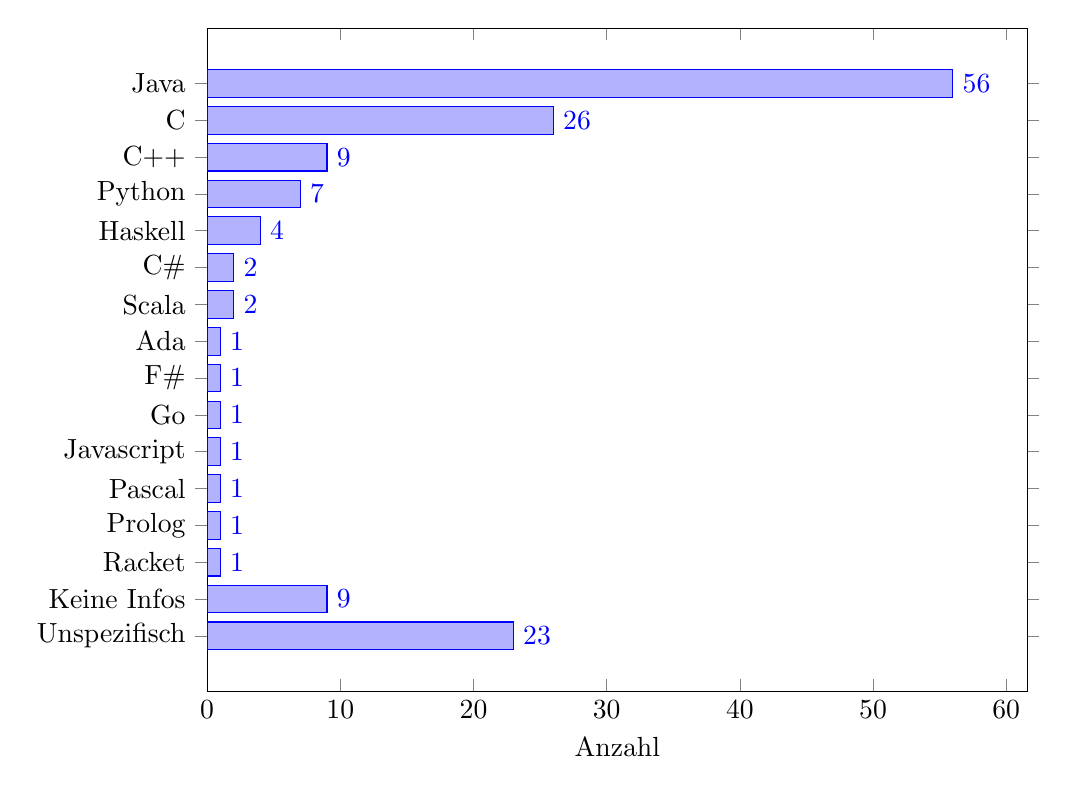
\begin{tikzpicture}
    \begin{axis}[
        xbar,
        width=12cm,
        height=10cm,
        symbolic y coords={{Unspezifisch}, {Keine Infos}, {Racket}, {Prolog}, {Pascal}, {Javascript}, {Go}, {F\#}, {Ada}, {Scala}, {C\#}, {Haskell}, {Python}, {C++},  {C}, {Java}},
        ytick=data,
        nodes near coords,
        xmin=0,
        xlabel={Anzahl}
    ]
        \addplot coordinates {
            (23,{Unspezifisch}) (9,{Keine Infos}) (1,{Racket}) (1,{Prolog}) (1,{Pascal}) (1,{Javascript}) (1,{Go}) (1,{F\#}) (1,{Ada}) (2,{Scala}) (2,{C\#}) (4,{Haskell}) (7,{Python})  (9,{C++}) (26,{C}) (56,{Java})
        };
    \end{axis}
\end{tikzpicture}

    \caption{Zahl der Programmiersprachen in Einführungskursen der Informatik}
\end{figure}

\begin{figure}[h!]
    \centering
    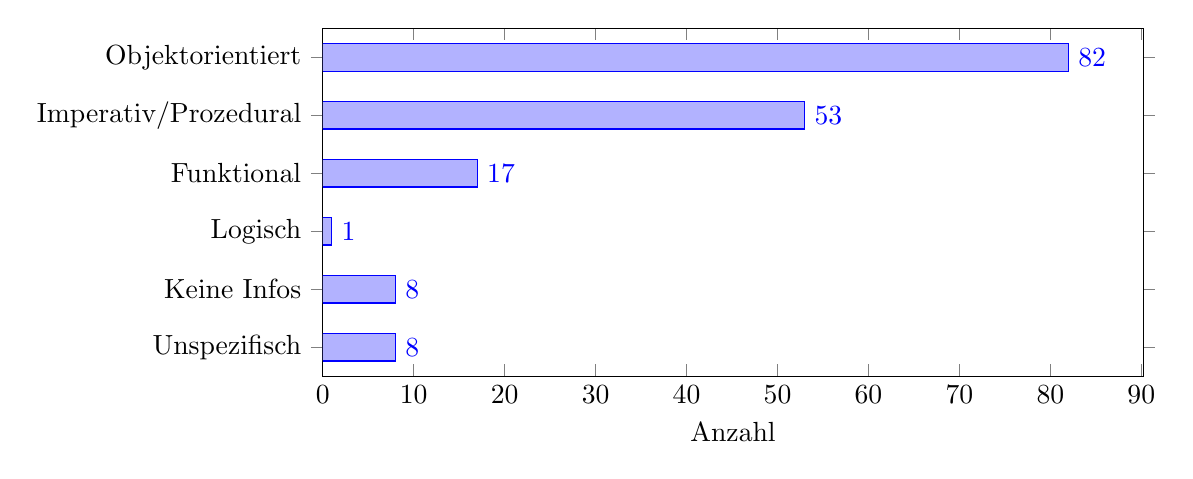
\begin{tikzpicture}
    \begin{axis}[
        xbar,
        width=12cm,
        height=6cm,
        symbolic y coords={{Unspezifisch}, {Keine Infos}, {Logisch}, {Funktional}, {Imperativ/Prozedural}, {Objektorientiert}},
        ytick=data,
        nodes near coords,
        xmin=0,
        xlabel={Anzahl}
    ]
        \addplot coordinates {
            (8,{Unspezifisch}) (8,{Keine Infos}) (1,{Logisch}) (17,{Funktional}) (53,{Imperativ/Prozedural}) (82,{Objektorientiert})
        };
    \end{axis}
\end{tikzpicture}
    \caption{Zahl der Paradigmen in Einführungskursen der Informatik}
\end{figure}